
The wide availability and reduced cost of molecular marker technology
has created opportunities to perform marker assisted selection of genotypes
in plant and animal breeding. Quantitative Trait Locus (QTL) mapping techniques
have proved useful for identifying markers genetically associated with genes 
conditioning agronomic phenotypes \citep{miles2008}. Using identified QTL to
support selection has grown in popularity as molecular marker data costs have 
decreased. Once a sufficient proportion of QTL-associated markers have been identified, 
the associated markers can be leveraged for making selections on a population. 
Individuals in a population genotyped for previously identified QTL-associated
markers can be selected based on the presence of desired alleles 
and/or haplotypes in a process known as Marker Assisted Selection (MAS).
MAS is usually effective on traits with a few large effect alleles with high 
heritability. However, when making selections on traits with many contributing genes 
with small effect distributed widely across a genome, MAS becomes less 
effective \citep{heffner2009}.

In order to apply MAS to traits with diverse genetic architectures, it is
advisable to combine MAS on juvenile individuals and subsequent phenotypic
selection on adults with favorable MAS scores \citep{lande1990}. This process, 
known as two-stage selection, has proven effective for improving
the coefficient of selection of breeding programs while avoiding expensive phenotypic
trials for individuals with low genetic potential. While inexpensive, two-stage selection 
only utilizes those markers associated with QTL with significant effects. The present cost of
genome wide SNP assays has fallen dramatically enough that today individuals are
frequently genotyped for hundreds, thousands, or even tens of thousands of SNPs. 
Information in SNPs that are not significantly associated with a trait are lost 
when applying MAS and two-stage selection, but may still have an small effect on the
expressed phenotype and thus could provide improved predictive 
accuracy of individual's genetic value.

Unlike QTL mapping and associated MAS techniques, genomic prediction methods
attempt to predict phenotypes utilizing all available SNP marker data collected 
from a population, allowing one of many possible statistical models to predict 
the marker-trait associations in a data driven way \citep{meuwissen2001}. 
The accuracy of genomic prediction relies on an appropriate choice of a 
statistical model to capture the relationship between the genetic architecture
of a trait and the underlying marker calls in a panel of high-density marker 
data. It is likely that the best statistical model for genomic prediction is 
dependent on the genetic architecture of
the predicted trait \citep{crossa2010, gonzalez-camacho2012, 
resende2012, cleveland2012, thavamanikumar2015}.  From a mathematical perspective,
models incorporating interactions between marker features have the 
capacity to achieve higher accuracy by capturing non-additive effects.
Experimental results support this hypothesis \citep{gonzalez-camacho2012}. 
Alternative prediction methods continue to be an active area of research 
in plant and animal breeding \citep{koning2012}.

% A more rapid transition into information about neural networks
% than is present in the lit review. This skips sections 
% describing selecting a particular model and of the fields of data science.
Concurrent with the advent of genomic selection as a practice the popularity of the 
interdisciplinary field known as data science has increased. Practitioners of data 
science apply machine learning and statistics to make predictions, usually
by applying ideas or techniques from a wide variety of domains 
including mathematics, physics, and computer science. Often, a data scientist's focus is to
create a predictive model than may not be associated with an underlying generative model. 
This can be viewed as the distinction between data science and classical statistics 
\citep{donoho2015, breiman2001}. The rapid increase in popularity of data science
is associated with better definitions of best practices for predictive modeling
across many disciplines as well as software packages to automate the 
process of building predictive models from any data source.

Neural networks are a type of model frequently employed by data scientists
for predictive modeling. Neural networks consist of layers of interconnected neurons
which map inputs to one or more outputs. Each neuron in a network can be expressed as a 
transformation of a weighted sum of $n$ inputs 

\begin{equation}
output_{lk} = \sum_{i=1}^{n} f_l(w_{lki} * x_{i} + b_{lk})
\label{eq:neuron}
\end{equation}

where $output_{lk}$ is the output from neuron $k$ in network layer $l$ having activation
function $f_l$, weights $w_{lki}$ and bias $b_{lk}$.

A neural network is a collection of neurons that map a 
length $n$ input vector $x = (x_1, ..., x_n)$ through a series of $j$ 
"hidden" layers $(l_1, ..., l_j)$. Each hidden layer consists of a variable 
number of neurons, each of which apply an associated coefficient, bias, and 
mathematical transformation to their input and forward the 
result on to every neuron in the subsequent layer forming an interconnected
network (Figure \ref{fig:deepnet}).

\ifdefined\showtablesandfigures
% A deep neural network with 3 hidden layers of varying sizes.

\def\layersep{1.5cm}

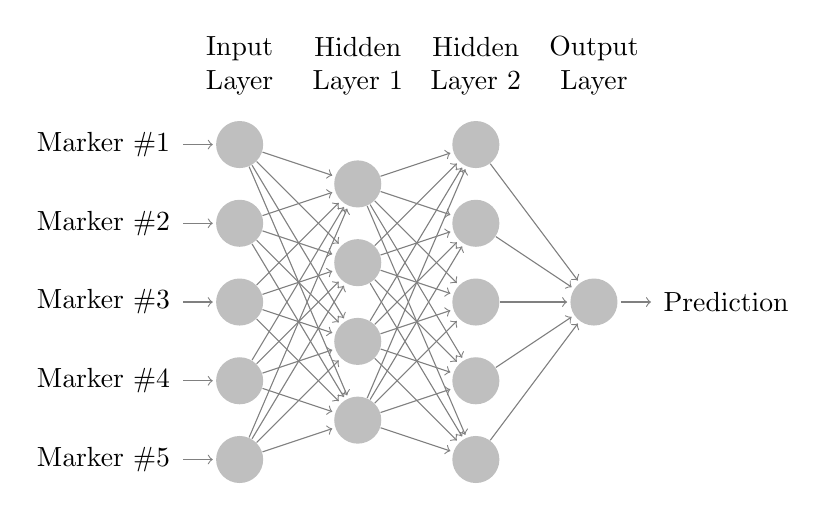
\begin{tikzpicture}[shorten >=1pt, ->, draw=black!50, node distance=\layersep]
    \tikzstyle{every pin edge}=[<-, shorten <=1pt]

    \tikzstyle{neuron}=[circle, fill=black!25,minimum size=17pt, inner sep=0pt]
    \tikzstyle{input neuron}=[neuron];
    \tikzstyle{output neuron}=[neuron];
    \tikzstyle{hidden neuron}=[neuron];

    \tikzstyle{annot}=[text width=4em, text centered]

    \foreach \name / \y in {1,...,5}
        \node[input neuron, pin=left:Marker \#\y] (I-\name) at (0,-\y) {};

    \foreach \name / \y in {1,...,4}
        \path[yshift=-0.5cm]
            node[hidden neuron] (H1-\name) at (\layersep * 1,-\y cm) {};

    \foreach \name / \y in {1,...,5}
        \path[yshift=0.0cm]
            node[hidden neuron] (H2-\name) at (\layersep * 2,-\y cm) {};

    \node[output neuron, pin={[pin edge={->}]right:Prediction}, right of=H2-3] (0) {};

    \foreach \source in {1,...,5}
        \foreach \dest in {1,...,4}
            \path (I-\source) edge (H1-\dest);

    \foreach \source in {1,...,4}
        \foreach \dest in {1,...,5}
            \path (H1-\source) edge (H2-\dest);

    \foreach \source in {1,...,5}
        \path (H2-\source) edge (0);

    \node[annot, above of=I-1, node distance=1cm] (il) {Input Layer};
    \node[annot, right of=il] (hl1) {Hidden Layer 1};
    \node[annot, right of=hl1] (hl2) {Hidden Layer 2};
    \node[annot, right of=hl2] {Output Layer};
\end{tikzpicture}

 % Label = fig:deepnet
\fi

Once the network is defined, it must be exposed to input and desired output
values, and adjusted to minimize error in output in a process known as training.
The weights and biases are often initialized by drawing from a
random normal distribution. From this initial state, error in 
the output of the network is propagated back through the hidden 
layers, and the weights and biases are updated in the direction that would 
decrease output error on many randomly drawn subsets of the input data. 
This turns the network training process into a general 
function minimization problem, where the parameters to the function are the 
weights and biases of the network neurons and the function to be 
minimized is the squared differences between the network outputs and 
the desired true values. The process of propagating output error back 
through a neural network is known as backpropagation, and has been used 
and improved extensively since its original description in the 
1980s \citep{rumelhart1986}.  Typically, the training data is split 
evenly into representative, randomly sampled collections of data 
called batches. The training algorithm exposes the network to each 
batch until they are depleted, after which the process is repeated. Each 
collection of batches is known as an epoch, and training typically
involves applying backpropagation for several hundred epochs, or until the network
weights and biases reach an equilibrium state that has converged to a 
globally minimum amount of prediction error.

%Good post, good links to the 'deep' part of deep nets.
%http://stats.stackexchange.com/questions/182734/what-is-the-difference-between-a-neural-network-and-a-deep-neural-network

It is trivial to add additional hidden layers to an existing neural network model.
Despite the ease of describing their architecture, networks with many hidden 
layers have been notoriously difficult to train. The amount of error
attributed to a neuron by backpropagation decreases in magnitude with each
additional layer added to the network. As a result, layers nearest the input train
very slowly in a phenomenon known as the vanishing gradient problem \citep{hochreiter1998}. 
Recently, a series of breakthroughs in neural network training along with well-known
increases in computer processing speeds have allowed efficient training
of deeper networks than were previously possible \citep{sutskever2013}.
A history of the deep learning literature is available in \cite{lecun2015}.
The increased training efficiency and potential to capture subtle
correlation relationships between two or more input features drove a need to 
differentiate these deeper networks from prior work, resulting in 
the emergence of the phrase "deep learning" to describe the construction 
and training of deep neural networks.

Previous attempts to apply neural networks to genomic prediction have resulted in 
an overfitting of the network to the training data and raised 
concerns about the computation time required to fit the model to datasets containing
many markers across many genotypes \citep{heslot2012, gonzalez-recio2014}. 
In retrospect, these results are not surprising. Multi-layer feedforward neural networks 
are capable of approximating functions of arbitrary complexity to arbitrary 
accuracy if provided enough neurons in even a single hidden 
layer. This property of neural networks is known as the 
universal approximation theorem, and can result in
overfitting if the weights of the network are not regularized in some way \citep{hornik1989}.

Given the promising results from regularized and Bayesian methods for
genomic prediction such as ridge or LASSO regression and the Bayesian family of regressors,
it is prudent to evaluate some of the many of neural network training algorithms which
incorporate regularization of weights during training. Today, networks based on these
and other regularization techniques continue to show success
across many domains \citep{schmidhuber2015}. Similarly, while neural networks are 
computationally demanding to train, the training algorithms 
themselves are often easily expressed with vector and matrix algebra. These algorithms are 
well suited to execution on Graphics Processing Unit (GPU) hardware, with reports 
of up to a sixty-fold speedup in training time \citep{sierra2010, schmidhuber2015}. 

To facilitate the evaluation of regularized neural networks, a neural 
network prediction model was implemented supporting two regularization
techniques. The first is a weight decay regularization which penalizes the 
weights $W$ with very large values similar to ridge regression \citep{krogh1992}.
The second is dropout regularization, in which a portion of neurons and 
their connections are removed at random during each training epoch, 
encouraging subsets of the network to learn to recognize input features 
independently. This allows neurons to adapt and build independently 
operating units, preventing the neurons from co-adapting and reducing 
overfitting \citep{srivastava2014}. In order to support training deep networks, 
network weights were initialized in a way that is known to cause
deep networks to converge to a global minimum error more rapidly \citep{glorot2010}. 
A modified form of backpropagation designed for deep network training 
was also selected \citep{dozat2015}. Finally, a divergence detection method and 
learning rate decay method were implemented to ensure models converged to
a global minimum error.

In this paper, we present the results of using this deep neural network
configuration to perform genomic prediction on three benchmark datasets 
from different species. A high and low heritability trait was selected 
from each dataset for a total of six genomic prediction tasks. A collection 
of regression techniques including single hidden layer and deep neural networks were 
applied to each task. We also quantitatively evaluate the 
time required to train neural networks using both CPU and GPU based 
network fitting. Last, we compare the performance of the regularized network
implementation with other available genomic prediction models in the collection.

% For the introduction, authors should be mindful of the broad readership of the journal.
% The introduction should set the stage for the importance of the work to a generalist 
% reader and draw the reader in to the specific study. The scope and impact of the 
% work should be clearly stated.

